\documentclass[12pt,a4paper]{article}

% =========================================================
% PACKAGE
% =========================================================
\usepackage[a4paper,margin=2.5cm]{geometry}
\usepackage[indonesian]{babel}
\usepackage[utf8]{inputenc}
\usepackage{textcomp}
\usepackage{amsmath,amssymb}
\usepackage{graphicx}
\usepackage{booktabs}
\usepackage{tabularx}
\usepackage{array}
\usepackage{enumitem}
\usepackage{float}
\usepackage{xcolor}
\usepackage{listings}
\usepackage{hyperref}
\usepackage{fancyhdr}
\setlength{\headheight}{21.42186pt}
\usepackage{tocloft}
\usepackage{indentfirst}
\usepackage{multirow}
\usepackage{placeins}
\usepackage[hypcap=false]{caption}

% =========================================================
% PENGATURAN UMUM
% =========================================================
\setlength{\parindent}{1.25cm}
\setlength{\parskip}{0.2cm}

\setlist[itemize]{leftmargin=1.2cm}
\setlist[enumerate]{leftmargin=1.2cm}

\hypersetup{
    colorlinks=true,
    linkcolor=black,
    urlcolor=blue,
    citecolor=black
}

\pagestyle{fancy}
\fancyhf{}
\lhead{\footnotesize \textit{Embedded Fuzzy Logic Control}}
\rhead{%
    \makebox[1.5cm][r]{%
        
\includegraphics[height=0.6cm]{images/Logo_FILKOM.png}%
        \hspace{0.03cm}%
        
\includegraphics[height=0.6cm]{images/Logo_Lab_RES.png}%
    }
}
\cfoot{\thepage}

\renewcommand{\headrulewidth}{0.4pt}
\renewcommand{\footrulewidth}{0pt}

% =========================================================
% PENGATURAN TABEL
% =========================================================
\newcolumntype{Y}{>{\centering\arraybackslash}X}
\newcolumntype{L}{>{\raggedright\arraybackslash}X}

\newcommand{\tableimage}[2]{%
    \includegraphics[
        height=#1,
        keepaspectratio
    ]{images/#2}%
}

% =========================================================
% PENGATURAN LISTING
% =========================================================
\lstset{
    basicstyle=\ttfamily\small,
    breaklines=true,
    frame=single,
    columns=fullflexible,
    keepspaces=true,
    showstringspaces=false
}

% =========================================================
% PLACEHOLDER GAMBAR
% =========================================================
\newcommand{\placeholderfigure}[2]{
    \begin{figure}[H]
        \centering
        \fbox{
            \begin{minipage}[c][#1][c]{0.88\textwidth}
                \centering
                \textbf{#2}
            \end{minipage}
        }
    \end{figure}
}

% =========================================================
% DOKUMEN
% =========================================================
\begin{document}

% =========================================================
% COVER
% =========================================================
\begin{titlepage}
    \thispagestyle{empty}
    \centering

    \vfill

    {\fontsize{16pt}{18pt}\selectfont\textbf{MODUL PERCOBAAN}\par}
    \vspace{0.5cm}

    {\LARGE \textbf{EMBEDDED FUZZY LOGIC CONTROL}\par}
    \vspace{0.3cm}

    {\large \textbf{Monitoring Kondisi Tanaman Hidroponik Berbasis ESP32}\par}

    \vspace{5cm}

    
\includegraphics[
        width=7cm,
        height=7cm
    ]{images/Logo_Universitas_Brawijaya.png}

    \vfill

    {\large Laboratorium Robotika dan Embedded System\par}
    {\large Fakultas Ilmu Komputer\par}
    {\large Universitas Brawijaya\par}
    {\large 2026\par}


\end{titlepage}

% =========================================================
% DAFTAR ISI
% =========================================================
\renewcommand{\cfttoctitlefont}{\hfill\Large\bfseries}
\renewcommand{\cftaftertoctitle}{\hfill}

\clearpage
\pagenumbering{roman}

\tableofcontents

\clearpage
\pagenumbering{arabic}
\pagenumbering{arabic}

% =========================================================
% 1. TUJUAN PERCOBAAN
% =========================================================
\section{Tujuan Percobaan}

Setelah mengikuti percobaan ini, penguji diharapkan dapat memahami alur sederhana pengambilan keputusan berbasis kondisi lingkungan tanaman. Penguji menggunakan data suhu dan kelembapan tanah sebagai masukan yang dibaca oleh mikrokontroler, kemudian mengolahnya menjadi keluaran indikator LED. Fokus kegiatan adalah menghubungkan data sensor, cara pengambilan keputusan, dan perilaku keluaran dalam satu sistem embedded sederhana.

Tujuan percobaan ini adalah:
\begin{enumerate}
    \item Memahami konsep dasar pengambilan keputusan menggunakan himpunan fuzzy.
    \item Memahami hubungan antara data sensor dan keluaran sistem.
    \item Menyusun kategori sederhana untuk input suhu dan kelembapan tanah.
    \item Menerapkan aturan pengambilan keputusan pada mikrokontroler.
    \item Mengamati perubahan keluaran berdasarkan perubahan kondisi input.
\end{enumerate}

% =========================================================
% 2. ALAT DAN BAHAN
% =========================================================
\section{Alat dan Bahan}

Alat dan bahan yang digunakan dalam percobaan ditunjukkan pada Tabel~\ref{tab:alatbahan1} dan Tabel~\ref{tab:alatbahan2}. Komponen digunakan sebagai media untuk membaca kondisi tanaman, mengolah data, dan menampilkan keputusan sistem.

% =========================================================
% TABEL ALAT DAN BAHAN BAGIAN 1
% =========================================================
\begin{center}
    \captionof{table}{Alat dan bahan percobaan}
    \label{tab:alatbahan1}

    \small
    \renewcommand{\arraystretch}{1.1}

    \begin{tabularx}{\textwidth}{c c L c L}
        \toprule
        \textbf{No.} &
        \textbf{Gambar} &
        \textbf{Alat/Bahan} &
        \textbf{Jumlah} &
        \textbf{Keterangan} \\
        \midrule

        1 &
        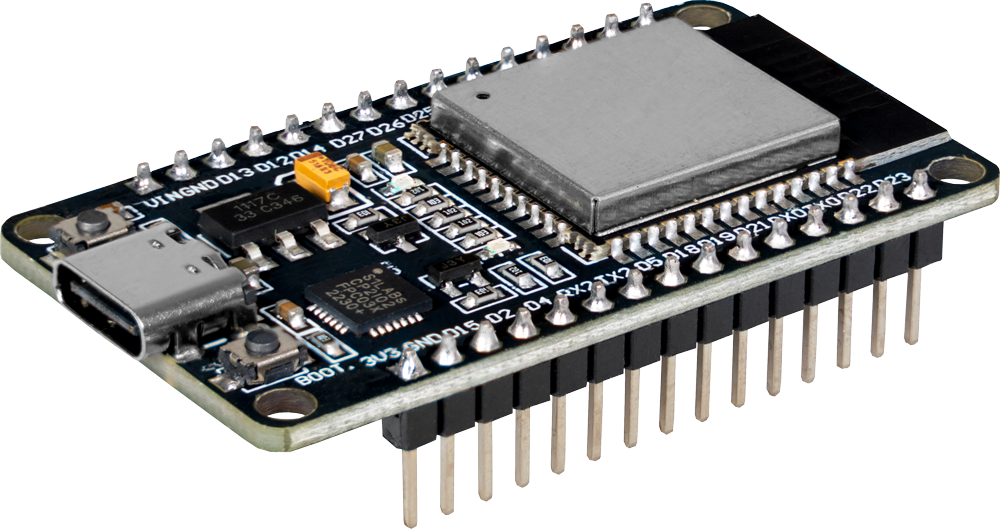
\includegraphics[
            width=1.8cm,
            height=1.1cm,
            keepaspectratio
        ]{images/esp32.png} &
        ESP32 &
        1 &
        Pengendali utama sistem \\

        2 &
        \raisebox{-0.5cm}{%
        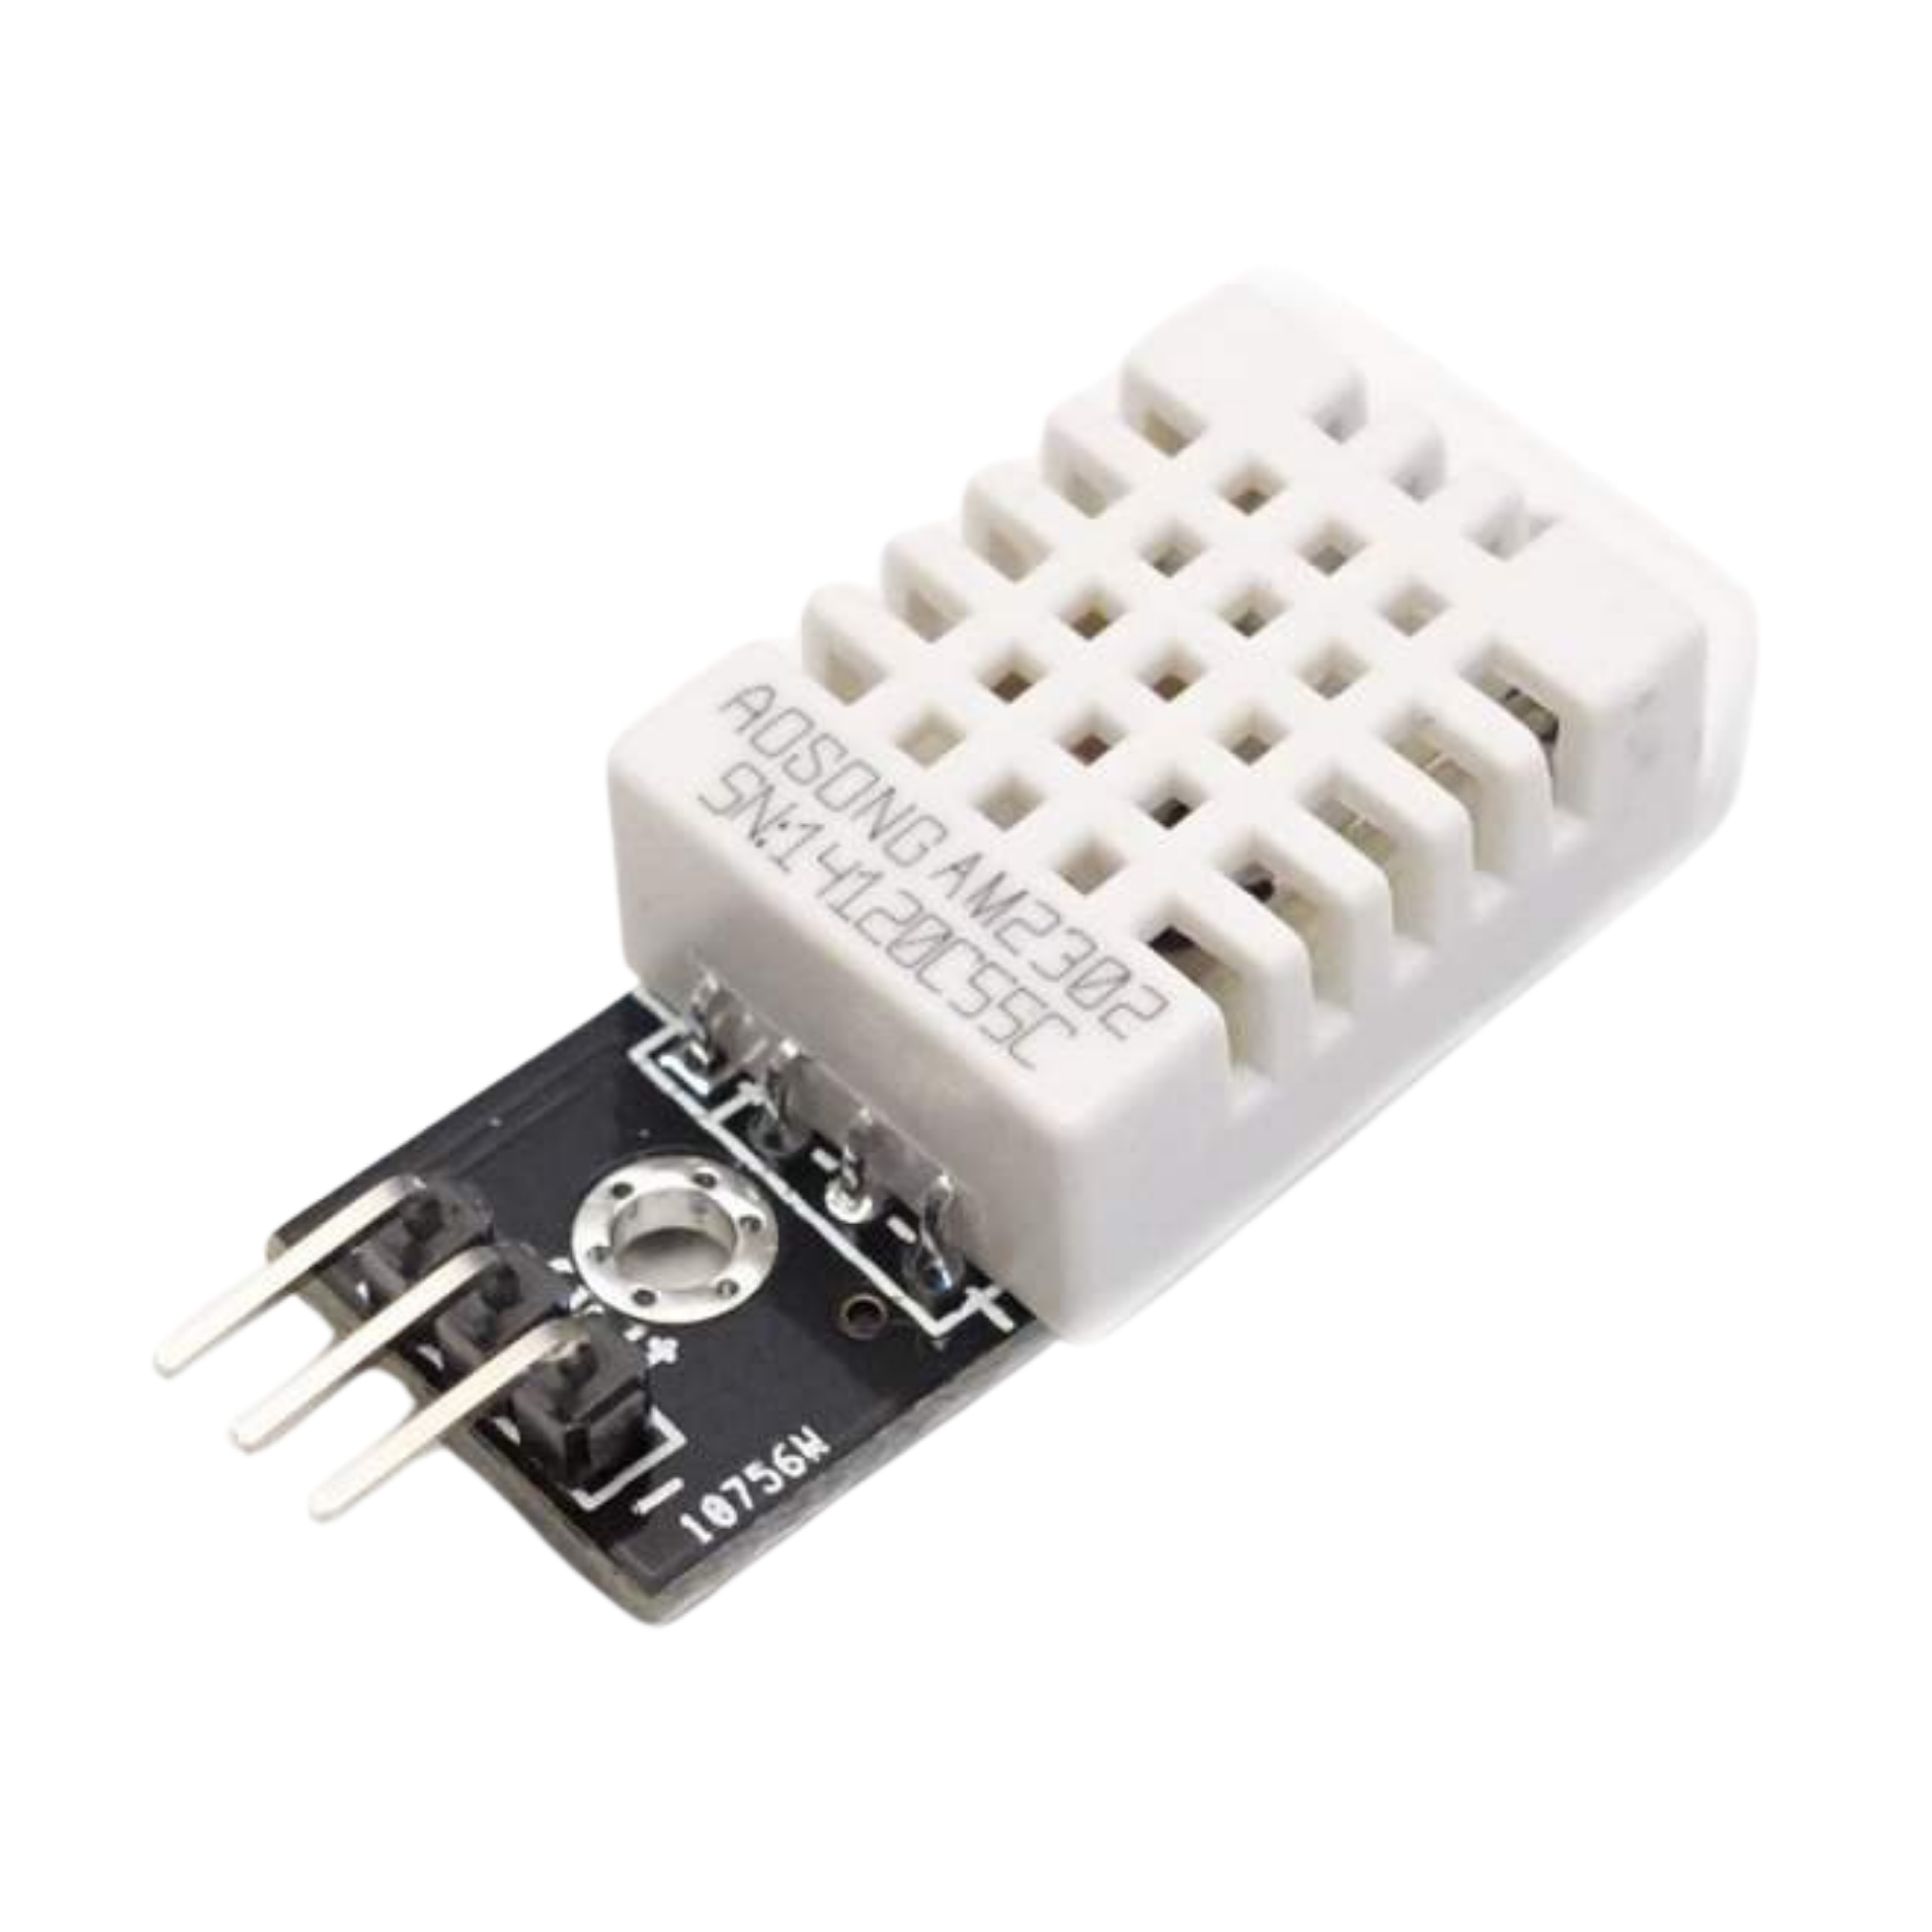
\includegraphics[
            width=1.8cm,
            height=1.1cm,
            keepaspectratio
        ]{images/dht22.png}%
        } &
        DHT22 &
        1 &
        Sensor suhu dan kelembapan udara \\

        3 &
    \raisebox{-0.5cm}{%
        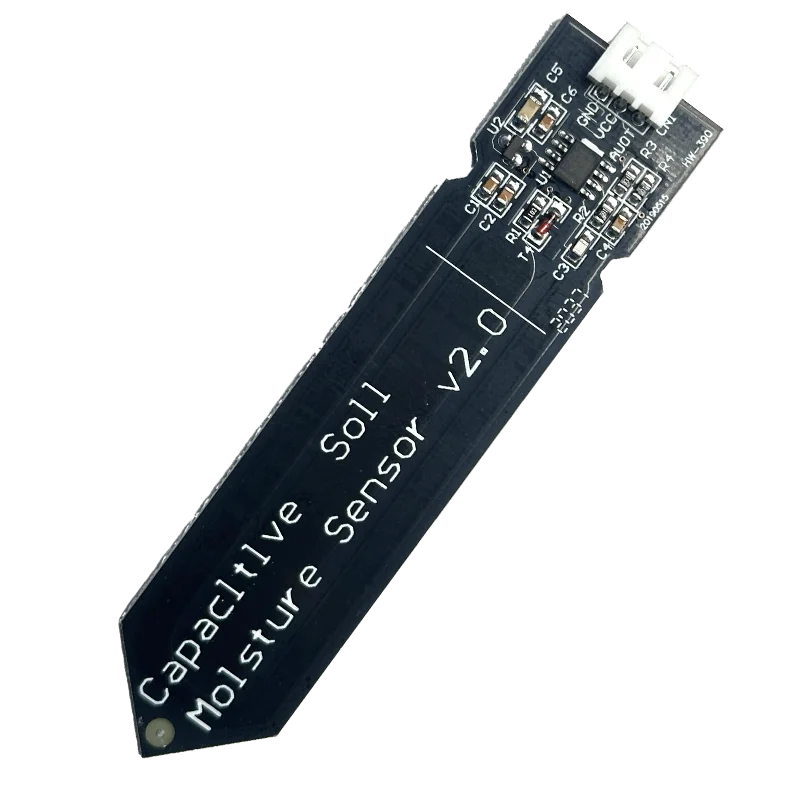
\includegraphics[
            width=1.8cm,
            height=1.1cm,
            keepaspectratio
        ]{images/soil-moisture.png}%
        } &
        Capacitive Soil Moisture Sensor &
        1 &
        Sensor kelembapan tanah/media \\

        % -------------------------------------------------
        % KABEL JUMPER
        % -------------------------------------------------
        4 &
        \multirow{3}{*}{
            \begin{minipage}[c][3.2cm][c]{2.2cm}
                \centering    
                \raisebox{0.5cm}{%
                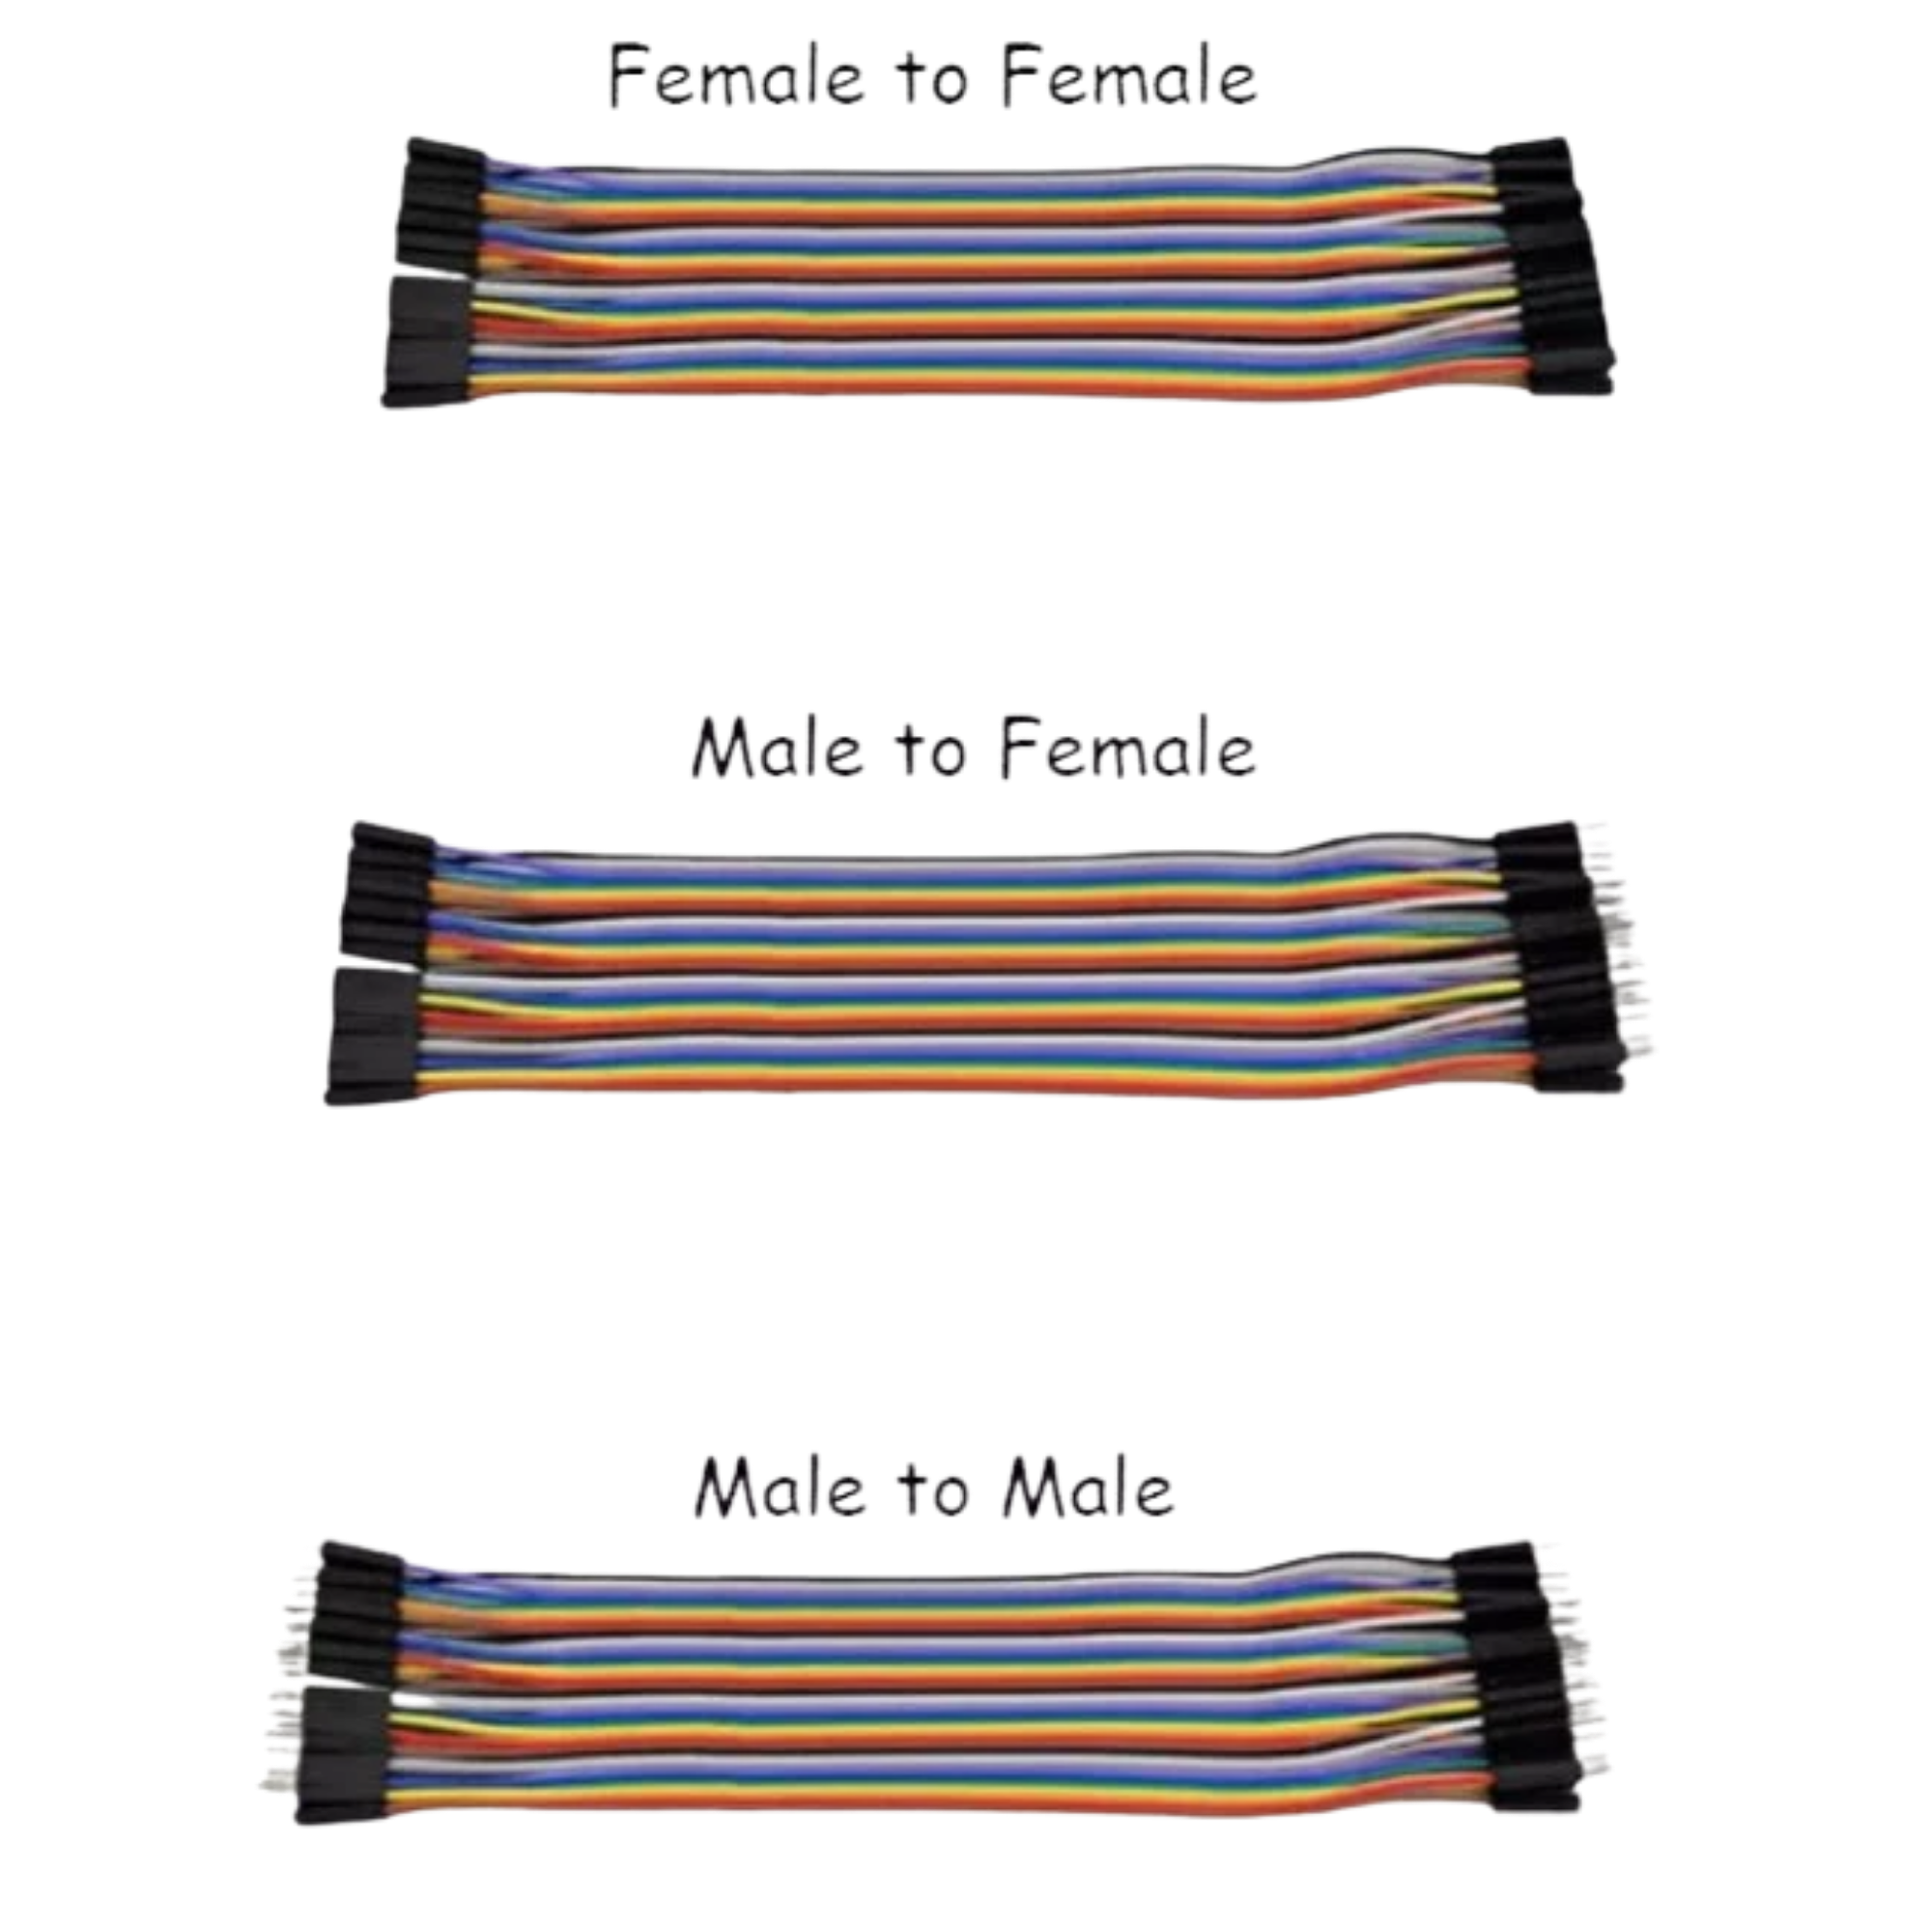
\includegraphics[
                    width=1.8cm,
                    height=2.8cm,
                    keepaspectratio
                ]{images/kabel-jumper.png}%
            }
            \end{minipage}
        } &
        \rule{0pt}{1cm}
        Kabel jumper F-F &
        Secukupnya &
        Penghubung komponen \\

        & &
        \rule{0pt}{1cm}
        Kabel jumper M-F &
        Secukupnya &
        Penghubung komponen \\

        & &
        \rule{0pt}{1cm}
        Kabel jumper M-M &
        Secukupnya &
        Penghubung komponen \\

        % -------------------------------------------------
        % BREADBOARD
        % -------------------------------------------------
        5 &
        \raisebox{-0.5cm}{%
        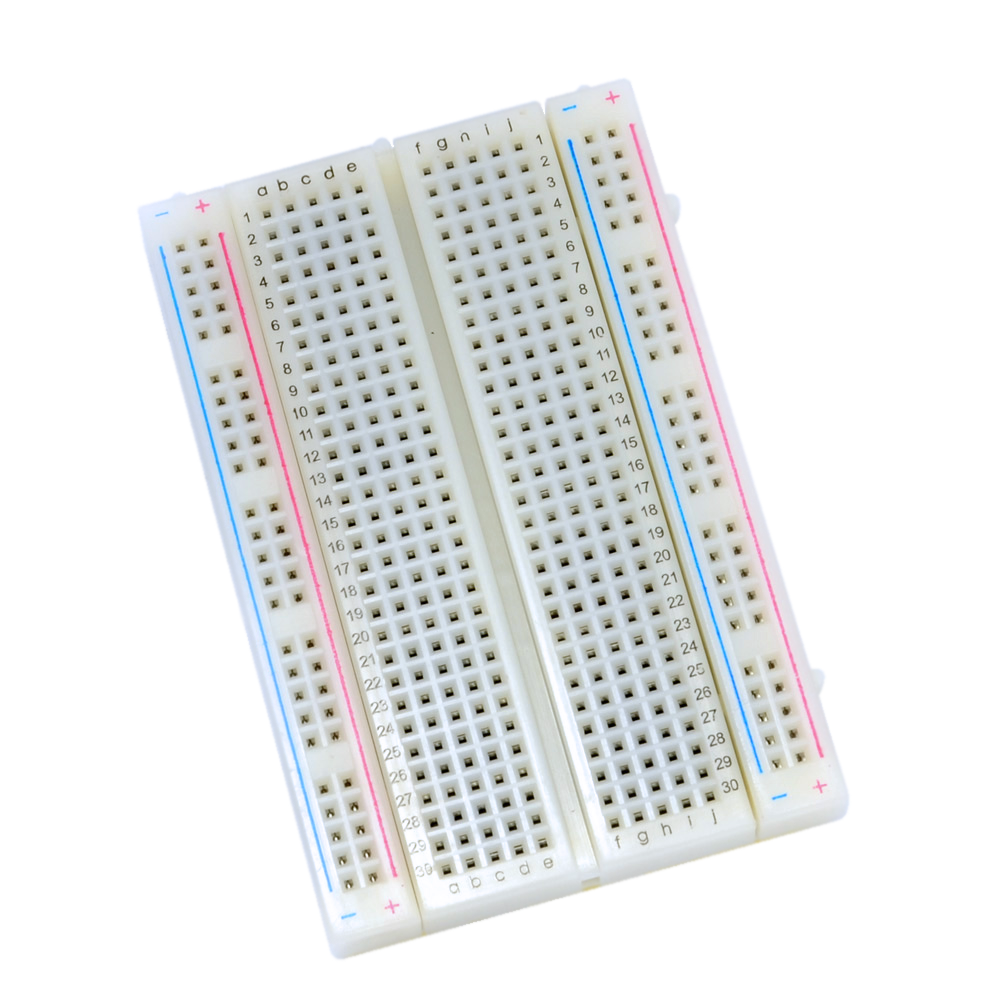
\includegraphics[
            width=1.8cm,
            height=1.1cm,
            keepaspectratio
        ]{images/bread_board.png}%
        } &
        Breadboard &
        1 &
        Media perakitan rangkaian \\

        \bottomrule
    \end{tabularx}
\end{center}

\vspace{0.3cm}

% =========================================================
% TABEL ALAT DAN BAHAN BAGIAN 2
% =========================================================
\begin{center}
    \captionof{table}{Alat dan bahan percobaan (lanjutan)}
    \label{tab:alatbahan2}

    \small
    \renewcommand{\arraystretch}{1.1}

    \begin{tabularx}{\textwidth}{c c L c L}
        \toprule
        \textbf{No.} &
        \textbf{Gambar} &
        \textbf{Alat/Bahan} &
        \textbf{Jumlah} &
        \textbf{Keterangan} \\
        \midrule

        % -------------------------------------------------
        % LED
        % -------------------------------------------------
        6 &
        \multirow{3}{*}{
            \begin{minipage}[c][3.2cm][c]{2.2cm}
                \centering
                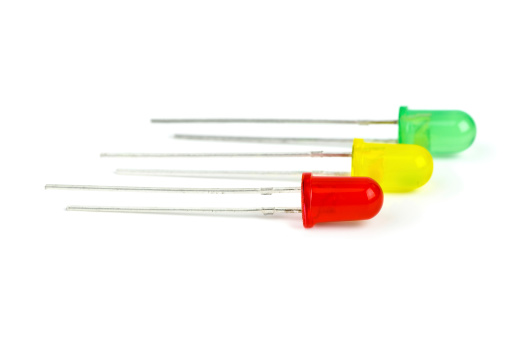
\includegraphics[
                    width=1.8cm,
                    height=2.8cm,
                    keepaspectratio
                ]{images/led.jpg}
            \end{minipage}
        } &
        \rule{0pt}{1cm}
        LED merah &
        1 &
        Indikator kondisi \\

        & &
        \rule{0pt}{1cm}
        LED kuning &
        1 &
        Indikator kondisi \\

        & &
        \rule{0pt}{1cm}
        LED hijau &
        1 &
        Indikator kondisi \\

        % -------------------------------------------------
        % KOMPONEN LAIN
        % -------------------------------------------------
        7 &
        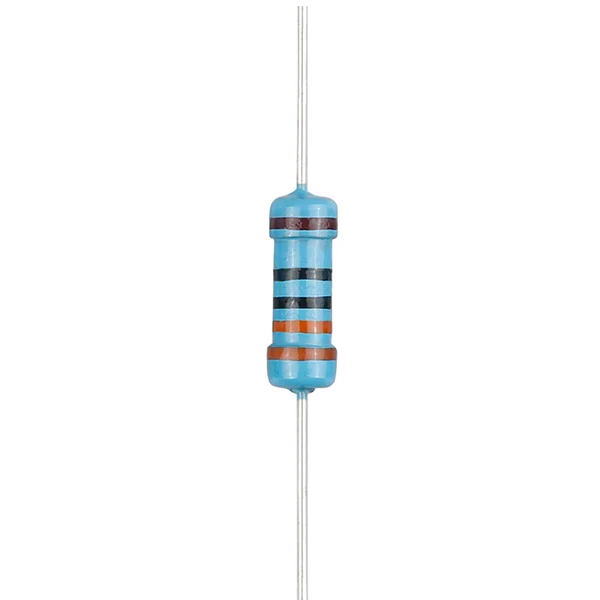
\includegraphics[
            width=1.8cm,
            height=1.1cm,
            keepaspectratio
        ]{images/resistor.png} &
        Resistor $330\,\Omega$ &
        3 &
        Pembatas arus LED \\

        8 &
        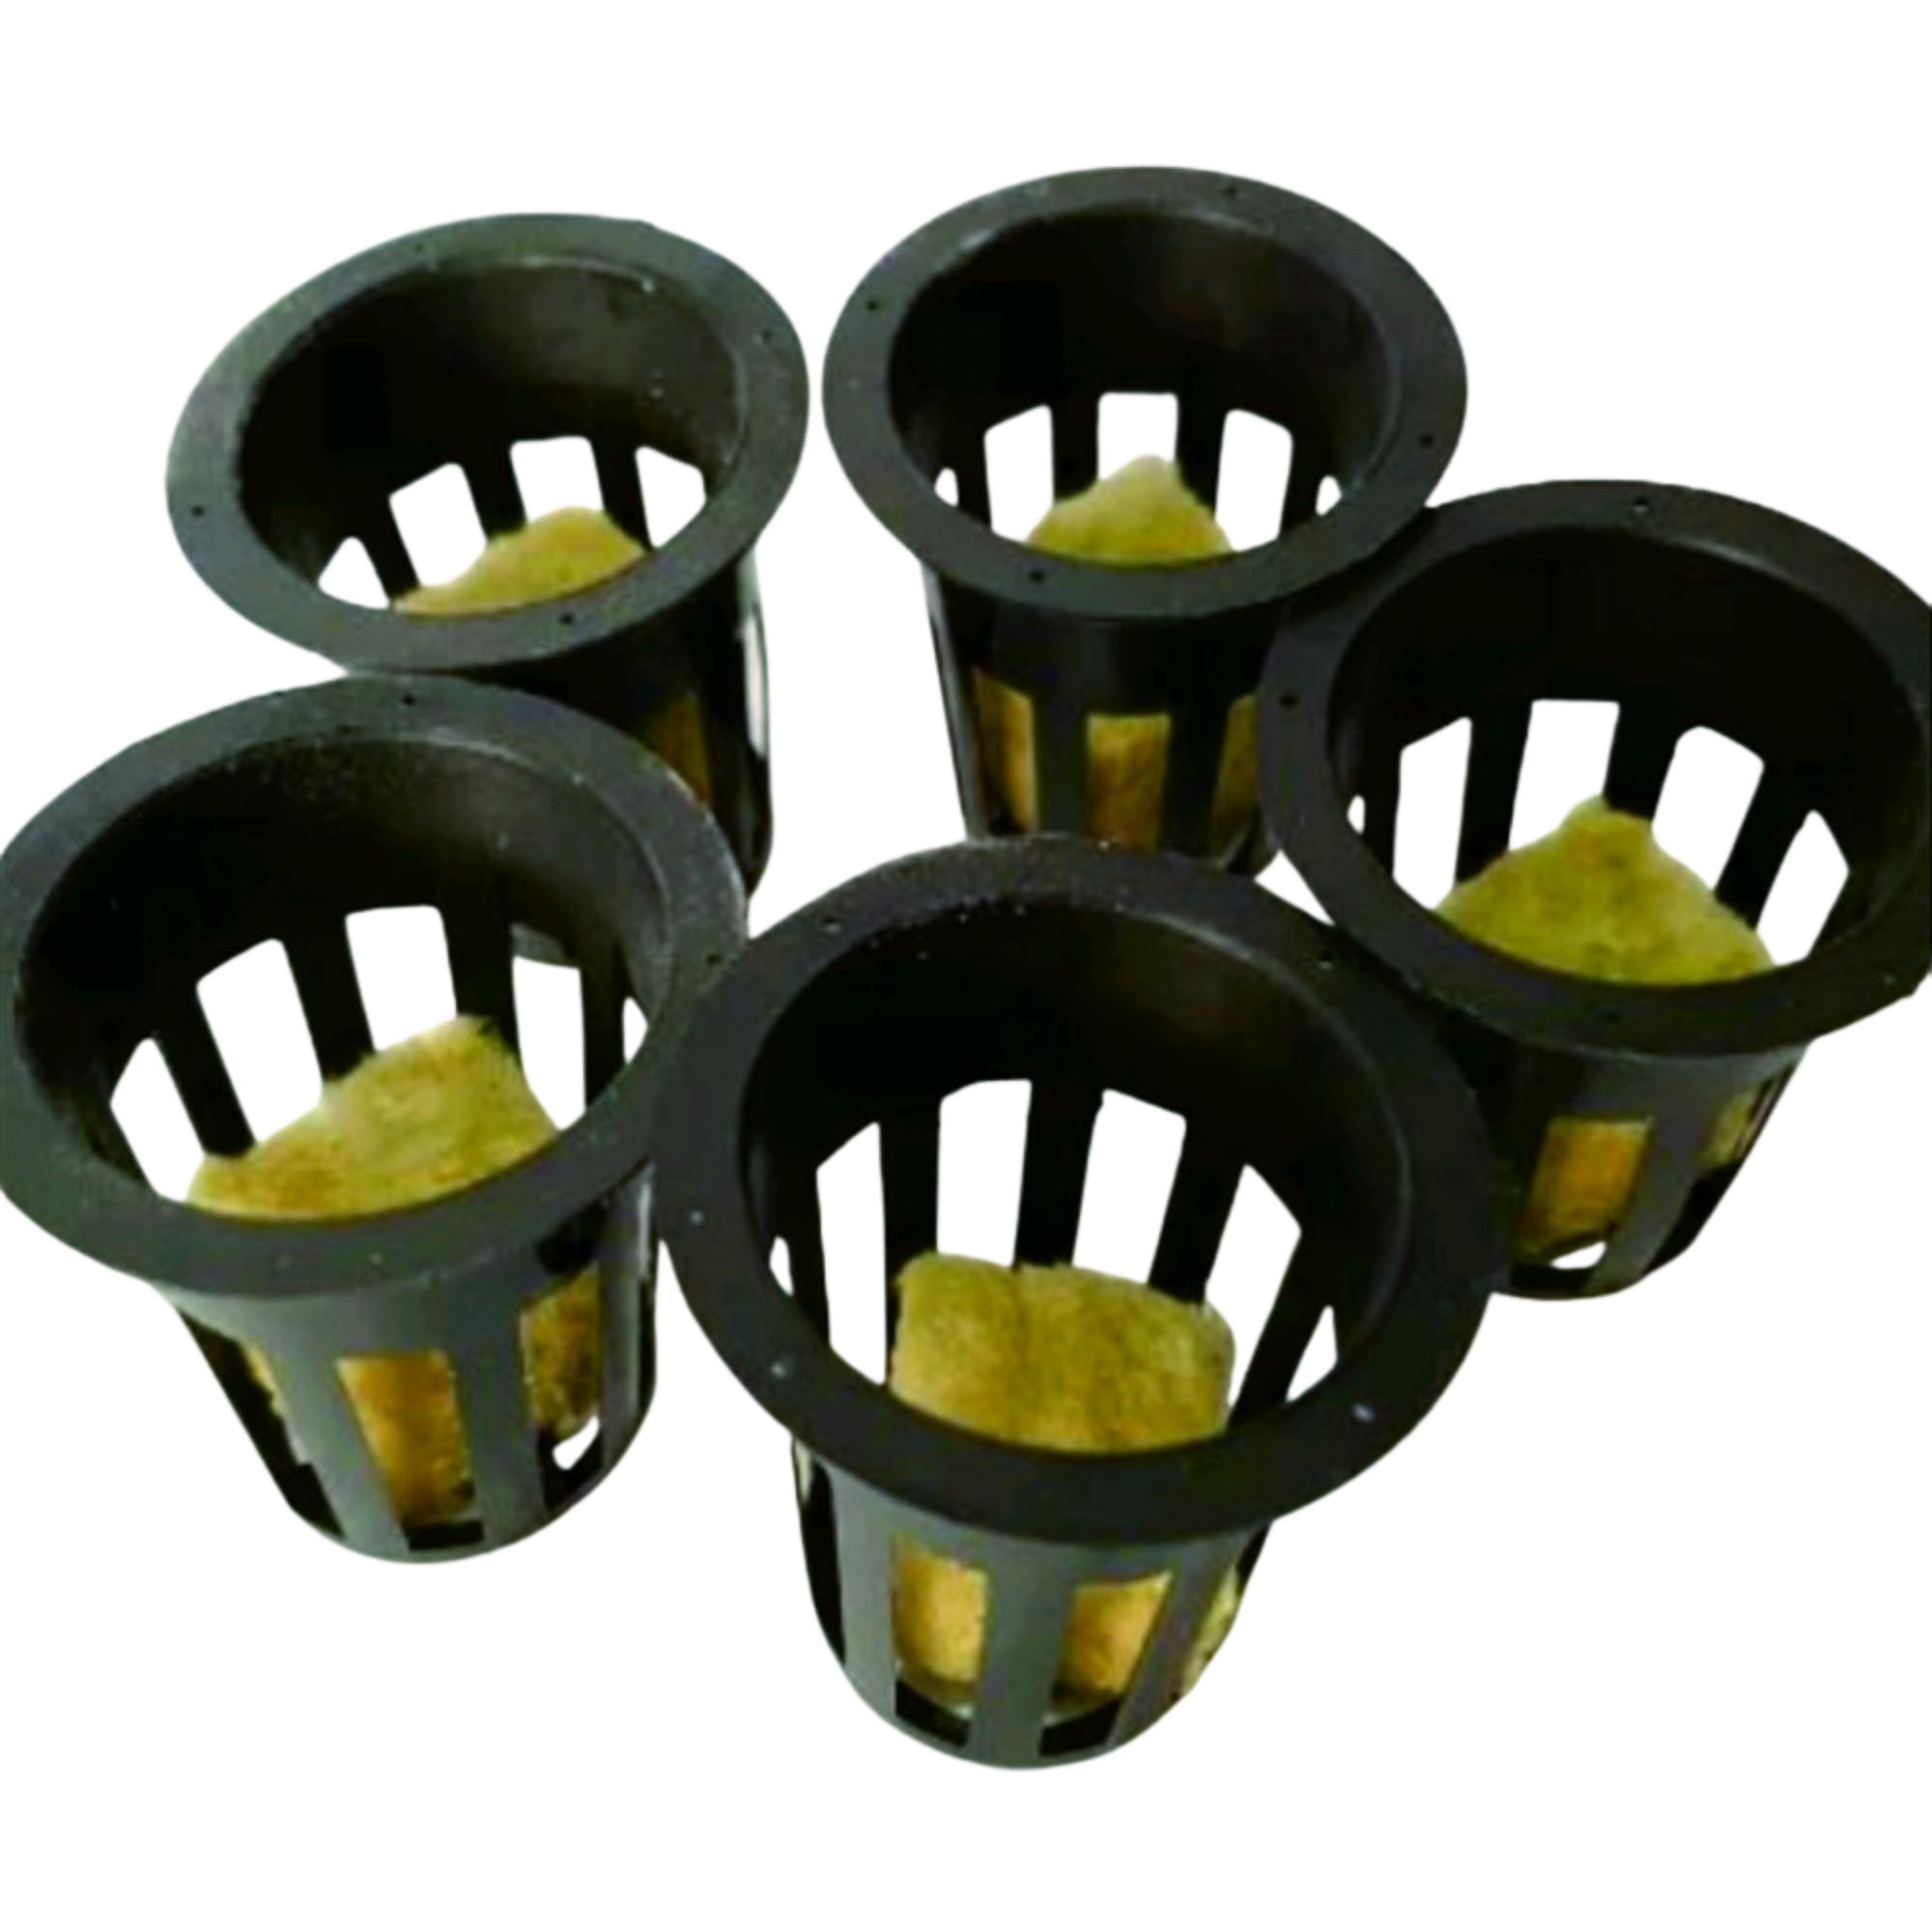
\includegraphics[
            width=1.8cm,
            height=1.1cm,
            keepaspectratio
        ]{images/hidroponik.png} &
        Paket hidroponik &
        1 &
        Objek pengamatan \\

        9 &
        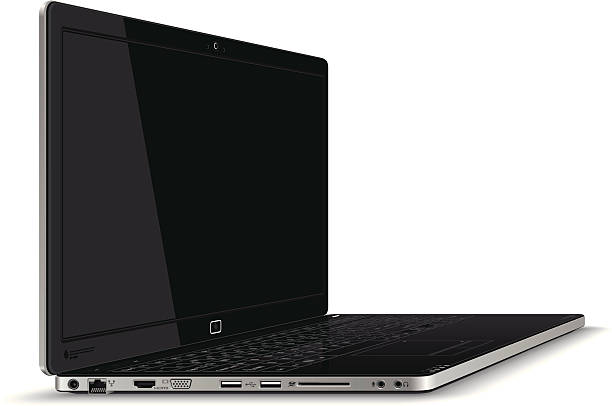
\includegraphics[
            width=1.8cm,
            height=1.1cm,
            keepaspectratio
        ]{images/laptop.jpg} &
        Laptop &
        1 &
        Pemrograman sistem \\

        \bottomrule
    \end{tabularx}
\end{center}

\FloatBarrier

% =========================================================
% 3. DASAR TEORI
% =========================================================
\section{Dasar Teori}

\subsection{Embedded System}

Embedded system adalah sistem komputer yang dibuat khusus untuk menjalankan fungsi tertentu di dalam sebuah perangkat. Sistem ini terdiri dari perangkat keras dan program yang saling bekerja untuk menerima data, mengolahnya, dan menghasilkan keluaran sesuai kebutuhan. Istilah embedded berarti sistem komputer tersebut menjadi bagian dari perangkat dan menjalankan fungsi yang sudah ditentukan. Pada percobaan ini, embedded system digunakan untuk membaca kondisi lingkungan tanaman melalui sensor suhu dan kelembapan tanah, kemudian memberikan indikasi kondisi melalui LED.

Berbeda dengan komputer umum yang dapat digunakan untuk berbagai keperluan, embedded system biasanya dirancang untuk satu atau beberapa fungsi tertentu. Pada percobaan ini, sistem bekerja dengan membaca nilai sensor, mengolah data tersebut, lalu menentukan kondisi tanaman berdasarkan hasil pembacaan.
\subsection{ESP32 sebagai Mikrokontroler}

Mikrokontroler adalah perangkat komputasi dalam satu chip yang memiliki unit pemrosesan, memori, dan antarmuka input-output untuk menjalankan fungsi kendali tertentu. Mikrokontroler dapat membaca masukan dari sensor, menjalankan program yang telah dibuat, dan mengendalikan perangkat keluaran. Kemampuan tersebut membuat mikrokontroler banyak digunakan pada sistem embedded.

ESP32 merupakan mikrokontroler yang digunakan sebagai pengendali utama pada percobaan ini. ESP32 menerima data dari DHT22 dan Capacitive Soil Moisture Sensor, kemudian menjalankan proses pengolahan berdasarkan program yang telah diunggah. Hasil pengolahan selanjutnya digunakan untuk menentukan kondisi LED sebagai keluaran sistem.

\subsection{Sensor}

Sensor adalah komponen yang digunakan untuk mendeteksi suatu besaran fisik dari lingkungan dan mengubahnya menjadi sinyal yang dapat dibaca oleh sistem. Data dari sensor menjadi masukan bagi mikrokontroler untuk menentukan kondisi yang sedang terjadi. Pada percobaan ini digunakan dua sensor dengan fungsi yang berbeda.

DHT22 digunakan untuk membaca suhu dan kelembapan udara. Nilai suhu digunakan sebagai salah satu parameter dalam proses pengambilan keputusan kondisi tanaman. Kelembapan udara dari DHT22 dapat ditampilkan sebagai informasi tambahan, tetapi pada rancangan utama percobaan ini input keputusan difokuskan pada suhu dan kelembapan tanah.

Capacitive Soil Moisture Sensor digunakan untuk mendeteksi tingkat kelembapan pada media tanam. Sensor menghasilkan nilai keluaran yang berubah sesuai kondisi media sehingga dapat digunakan sebagai masukan sistem. Nilai tersebut kemudian dikelompokkan ke dalam kategori seperti kering, sedang, dan lembap.

\subsection{Aktuator}

Aktuator adalah komponen yang mengubah sinyal kendali dari sistem menjadi suatu aksi atau keluaran fisik. Dengan kata lain, aktuator merupakan bagian yang melakukan tindakan berdasarkan keputusan yang dihasilkan oleh pengendali. Contoh aktuator pada dalam kehidupan sehari-hari antara lain lampu yang menyala, kipas yang berputar, atau buzzer yang berbunyi.

Pada percobaan ini, LED digunakan sebagai keluaran indikator sistem. LED tidak melakukan gerakan mekanis seperti motor, tetapi dapat digunakan sebagai aktuator sederhana untuk memberikan respons visual terhadap keputusan sistem. Tiga LED digunakan untuk menunjukkan kondisi yang berbeda, yaitu merah untuk kondisi kurang sesuai, kuning untuk kondisi yang perlu diperhatikan, dan hijau untuk kondisi relatif baik.

\subsection{Konsep Dasar Fuzzy Logic}

Fuzzy logic adalah metode pengambilan keputusan yang memungkinkan sistem menangani kondisi yang tidak selalu memiliki batas yang pasti. Berbeda dengan sistem yang hanya menggunakan keputusan “ya” atau “tidak”, fuzzy logic dapat mengenali kondisi di antara keduanya berdasarkan tingkat kecocokan suatu nilai. Misalnya, suhu 27°C tidak harus langsung dianggap hanya sebagai suhu sedang atau panas. Suhu tersebut dapat dikatakan cukup sedang dan sebagian panas, karena masih memiliki tingkat kecocokan terhadap kedua kategori tersebut.

Tingkat kecocokan suatu nilai terhadap suatu kategori disebut derajat keanggotaan. Nilainya berada antara 0 sampai 1. Nilai 0 berarti suatu nilai tidak sesuai dengan kategori tersebut, sedangkan nilai 1 berarti nilai tersebut sepenuhnya sesuai. Nilai di antara 0 dan 1 menunjukkan bahwa nilai tersebut hanya sebagian sesuai dengan kategori tersebut.

Untuk menentukan derajat keanggotaan, digunakan membership function. Membership function berfungsi untuk menentukan seberapa besar suatu nilai sensor termasuk ke dalam kategori tertentu. Bentuk membership function yang sederhana dapat berupa segitiga atau trapesium. Pada percobaan ini digunakan membership function berbentuk segitiga karena sederhana dan mudah digunakan untuk membagi nilai sensor ke dalam beberapa kategori.

Untuk fungsi segitiga, derajat keanggotaan dapat dihitung menggunakan persamaan:

\[
\mu(x)=
\begin{cases}
0, & x\leq a \\
\dfrac{x-a}{b-a}, & a < x \leq b \\
\dfrac{c-x}{c-b}, & b < x < c \\
0, & x\geq c
\end{cases}
\]

Sebagai contoh, misalkan sensor membaca suhu $27^\circ$C. Berdasarkan
membership function, suhu tersebut termasuk dalam kategori sedang dan panas.
Untuk kategori sedang dengan parameter $[20,25,30]$, derajat keanggotaannya
dihitung sebagai:

\[
\mu_{\text{sedang}}(27)
=
\frac{30-27}{30-25}
=
0,6
\]

Sementara itu, untuk kategori panas dengan parameter $[25,30,35]$:

\[
\mu_{\text{panas}}(27)
=
\frac{27-25}{30-25}
=
0,4
\]

Dengan demikian, suhu $27^\circ$C memiliki derajat keanggotaan sebesar $0,6$
pada kategori sedang dan $0,4$ pada kategori panas. Pada saat yang sama,
misalkan hasil pembacaan sensor menunjukkan bahwa kelembapan tanah berada
sepenuhnya pada kategori sedang. Oleh karena itu, derajat keanggotaannya pada
kategori tersebut adalah $1,0$. Nilai $1,0$ menunjukkan tingkat keanggotaan
penuh, bukan nilai kelembapan tanah yang sebenarnya. Dengan kondisi tersebut,
dua rule dapat aktif.

Setelah nilai sensor diubah menjadi derajat keanggotaan melalui proses fuzzifikasi, sistem masuk ke tahap inferensi. Pada tahap ini, sistem menggunakan aturan atau rule berbentuk IF–THEN untuk menentukan keputusan. Misalnya, terdapat aturan “IF suhu sedang AND kelembapan tanah sedang THEN kondisi hijau”. Untuk aturan yang menggunakan AND, derajat keanggotaan yang digunakan adalah nilai terkecil atau minimum. Sebaliknya, pada aturan yang menggunakan OR, nilai yang digunakan adalah nilai terbesar atau maksimum.

Rule pertama adalah “IF suhu sedang AND kelembapan tanah sedang THEN hijau”. Karena menggunakan AND, kekuatan rule diambil dari nilai minimum, yaitu:

\[
\alpha_1 = \min(0{,}6;1{,}0)=0{,}6
\]

Rule kedua adalah “IF suhu panas AND kelembapan tanah sedang THEN kuning”. Kekuatan rule tersebut adalah:

\[
\alpha_2 = \min(0{,}4;1{,}0)=0{,}4
\]

Dengan demikian, kedua rule tetap ikut memengaruhi keputusan. Rule pertama memiliki kekuatan 0,6, sedangkan rule kedua memiliki kekuatan 0,4. Hal ini menunjukkan bahwa fuzzy logic tidak hanya memilih kategori dengan nilai keanggotaan terbesar, tetapi tetap mempertimbangkan kategori lain yang memiliki derajat keanggotaan.

Setelah proses inferensi selesai, sistem masuk ke tahap defuzzifikasi, yaitu proses mengubah hasil dari rule yang aktif menjadi satu nilai keluaran akhir. Pada percobaan ini digunakan nilai keluaran representatif berupa 0 untuk merah, 50 untuk kuning, dan 100 untuk hijau. Nilai tersebut kemudian digabungkan berdasarkan kekuatan masing-masing rule menggunakan metode rata-rata berbobot.

Berdasarkan contoh sebelumnya, rule pertama menghasilkan keluaran hijau dengan kekuatan 0,6, sedangkan rule kedua menghasilkan keluaran kuning dengan kekuatan 0,4. Maka, nilai keluaran akhir pada tahap defuzzifikasi dihitung sebagai berikut:

\[
z = \frac{\sum_{i=1}^{n} \alpha_i z_i}{\sum_{i=1}^{n} \alpha_i}
\]

dengan:
\begin{itemize}
    \item $z$ = nilai keluaran akhir,
    \item $\alpha_i$ = kekuatan \textit{rule} ke-$i$,
    \item $z_i$ = nilai keluaran dari \textit{rule} ke-$i$.
\end{itemize}

Maka:
\begin{align}
z &= \frac{(0,6 \times 100) + (0,4 \times 50)}
         {0,6 + 0,4} \\
  &= \frac{60 + 20}{1} \\
  &= 80
\end{align}

Nilai 80 merupakan hasil defuzzifikasi atau nilai keluaran akhir sistem. Nilai tersebut kemudian dipetakan ke kategori LED berdasarkan rentang yang telah ditentukan, misalnya 0–24 untuk merah, 25–74 untuk kuning, dan 75–100 untuk hijau. Dengan demikian, nilai 80 menghasilkan LED hijau.

\begin{figure}[H]
    \centering
    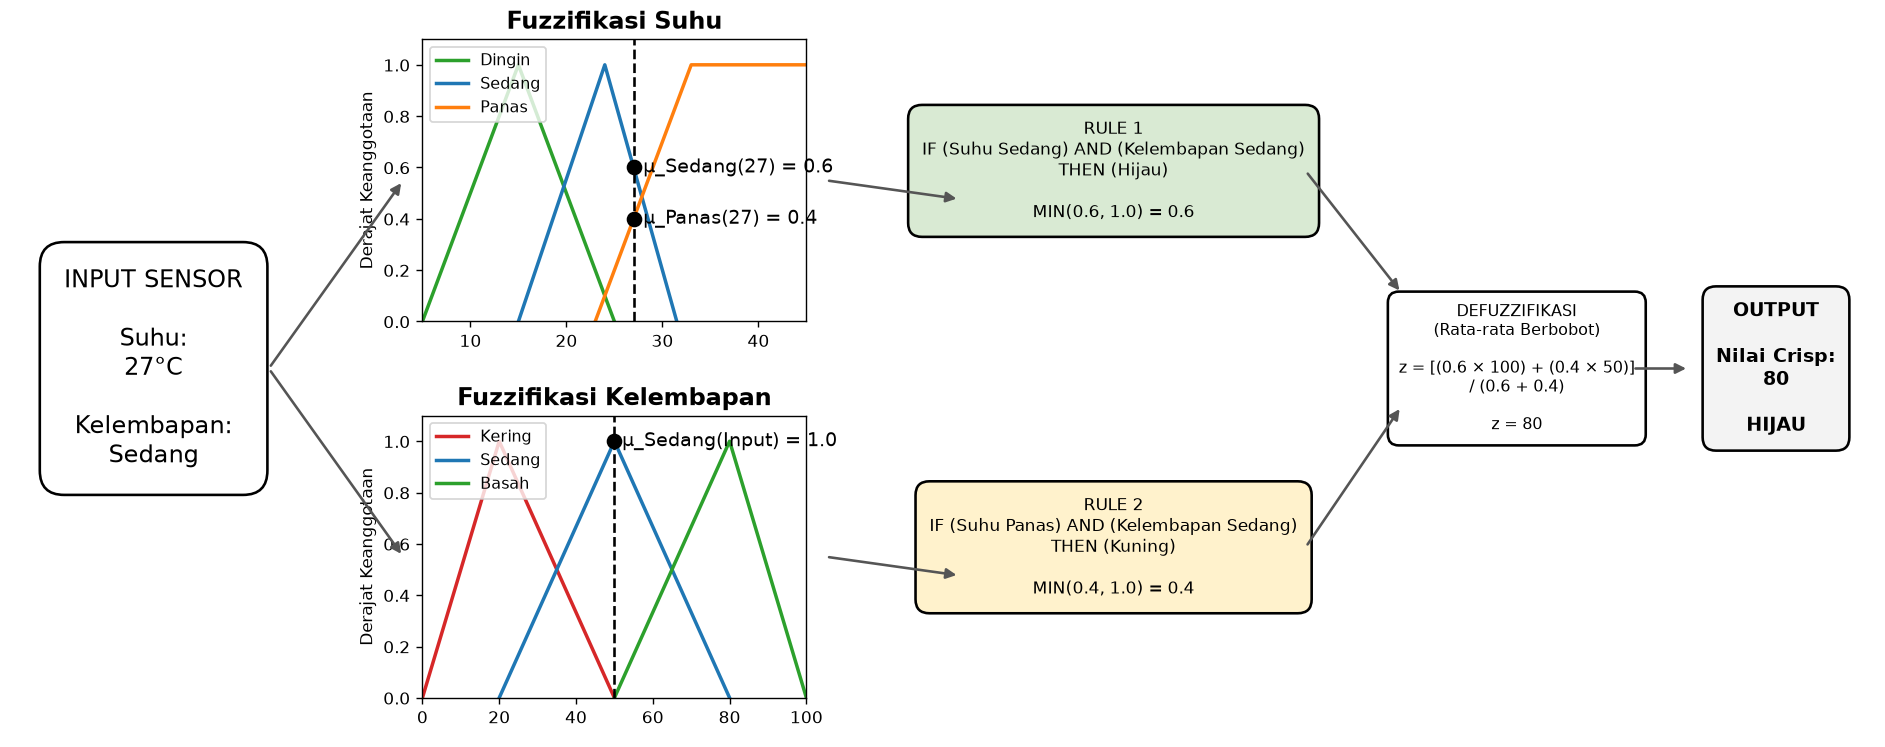
\includegraphics[width=\textwidth]{images/alur-contoh.png}
    \caption{Alur sederhana proses fuzzy logic}
    \label{fig:alur-fuzzy}
\end{figure}

\subsection{Direct Fuzzy Logic Control}

Direct Fuzzy Logic Control adalah metode pengambilan keputusan yang langsung menggunakan hasil pengolahan fuzzy untuk menentukan keluaran sistem. Dalam penerapannya, nilai dari sensor suhu dan kelembapan tanah diproses menggunakan fuzzy logic untuk menentukan kondisi sistem yang kemudian ditampilkan melalui LED. Pendekatan yang digunakan adalah Direct Fuzzy Logic Control, sehingga fuzzy logic berperan secara langsung dalam menentukan keluaran berdasarkan kondisi sensor. Sementara itu, pendekatan fuzzy logic yang dikombinasikan dengan pengendali lain, seperti PI atau PID, tidak menjadi bagian dari pembahasan.

Secara sederhana, prosesnya dimulai dari pembacaan nilai sensor. Nilai tersebut kemudian diubah menjadi derajat keanggotaan melalui proses fuzzifikasi. Setelah itu, sistem menjalankan rule yang telah dibuat pada tahap inferensi. Hasil dari rule kemudian diolah melalui defuzzifikasi untuk mendapatkan satu nilai keluaran akhir.
\[
\text{Nilai Sensor}
\rightarrow
\text{Fuzzy Logic}
\rightarrow
\text{Keluaran}
\rightarrow
\text{LED}
\]

Perubahan suhu atau kelembapan tanah dapat memengaruhi keluaran karena perubahan tersebut dapat mengubah derajat keanggotaan dan rule yang aktif. Hasil akhirnya ditampilkan melalui LED sehingga hubungan antara perubahan kondisi sensor dan keputusan sistem dapat diamati secara langsung.

% =========================================================
% 4. PERSIAPAN PERCOBAAN
% =========================================================
\section{Persiapan Percobaan}

Sebelum memulai percobaan, pastikan laptop, perangkat lunak, dan komponen yang digunakan telah siap. Ikuti konfigurasi berikut sebelum melakukan perakitan dan pengunggahan program.

\subsection{Persiapan Perangkat Lunak}

Perangkat lunak yang digunakan dalam percobaan adalah Arduino IDE. Arduino IDE digunakan untuk menulis program, memilih board ESP32, memilih port komunikasi, mengunggah program ke mikrokontroler, dan memantau data melalui Serial Monitor.

Pastikan Arduino IDE telah ter-install pada laptop sebelum percobaan dimulai. Gunakan versi terbaru yang dapat diunduh melalui situs resmi Arduino pada tautan berikut: \url{https://www.arduino.cc/en/software/}.

\begin{enumerate}
    \item Buka situs resmi Arduino dan unduh Arduino IDE sesuai dengan sistem operasi yang digunakan.
    \item Install Arduino IDE pada laptop.
    \item Buka Arduino IDE dan pastikan program dapat dijalankan.
\end{enumerate}

\subsection{Board Package dan Library}

Program membutuhkan board package dan library agar Arduino IDE dapat mengenali perangkat dan menjalankan fungsi sensor. Board package digunakan agar Arduino IDE dapat melakukan proses kompilasi dan pengunggahan program ke ESP32. Library digunakan untuk menyediakan fungsi komunikasi dan pembacaan sensor yang diperlukan oleh program.

\begin{enumerate}
    \item Buka Arduino IDE.
    \item Masuk ke \textbf{File} $\rightarrow$ \textbf{Preferences}.
    \item Pada bagian \textbf{Additional Boards Manager URLs}, tambahkan URL berikut:
    
    \url{https://espressif.github.io/arduino-esp32/package_esp32_index.json}
    
    \item Buka \textbf{Tools} $\rightarrow$ \textbf{Board} $\rightarrow$ \textbf{Boards Manager}.
    \item Cari \textbf{esp32} dan install \textbf{esp32 by Espressif Systems}.
    \item Setelah proses instalasi selesai, pilih \textbf{ESP32 Dev Module} melalui \textbf{Tools} $\rightarrow$ \textbf{Board}.    \item Hubungkan ESP32 ke laptop menggunakan kabel USB.
    \item Pilih port komunikasi ESP32 melalui \textbf{Tools} $\rightarrow$ \textbf{Port}.
\end{enumerate}

Library yang dibutuhkan dalam percobaan dapat di-install melalui Arduino IDE. Buka
\textbf{Tools} $\rightarrow$ \textbf{Manage Libraries}. Pada kolom pencarian, masukkan
nama library yang dibutuhkan, kemudian pilih library yang sesuai dan klik
\textbf{Install}. Library yang digunakan dalam percobaan adalah:

\begin{table}[H]
    \centering
    \caption{Library yang digunakan}
    \label{tab:library}
    \begin{tabularx}{\textwidth}{c L L}
        \toprule
        \textbf{No.} &
        \textbf{Library} &
        \textbf{Fungsi} \\
        \midrule
        1 &
        DHT Sensor Library &
        Membaca data suhu dan kelembapan dari sensor DHT22 \\

        2 &
        Adafruit Unified Sensor &
        Library pendukung yang dibutuhkan oleh DHT Sensor Library \\
        \bottomrule
    \end{tabularx}
\end{table}

Pastikan seluruh library yang dibutuhkan telah berhasil terpasang sebelum program diunggah ke ESP32.

% =========================================================
% 5. PERANCANGAN SISTEM
% =========================================================
\section{Perancangan Sistem}

\begin{figure}[H]
    \centering
    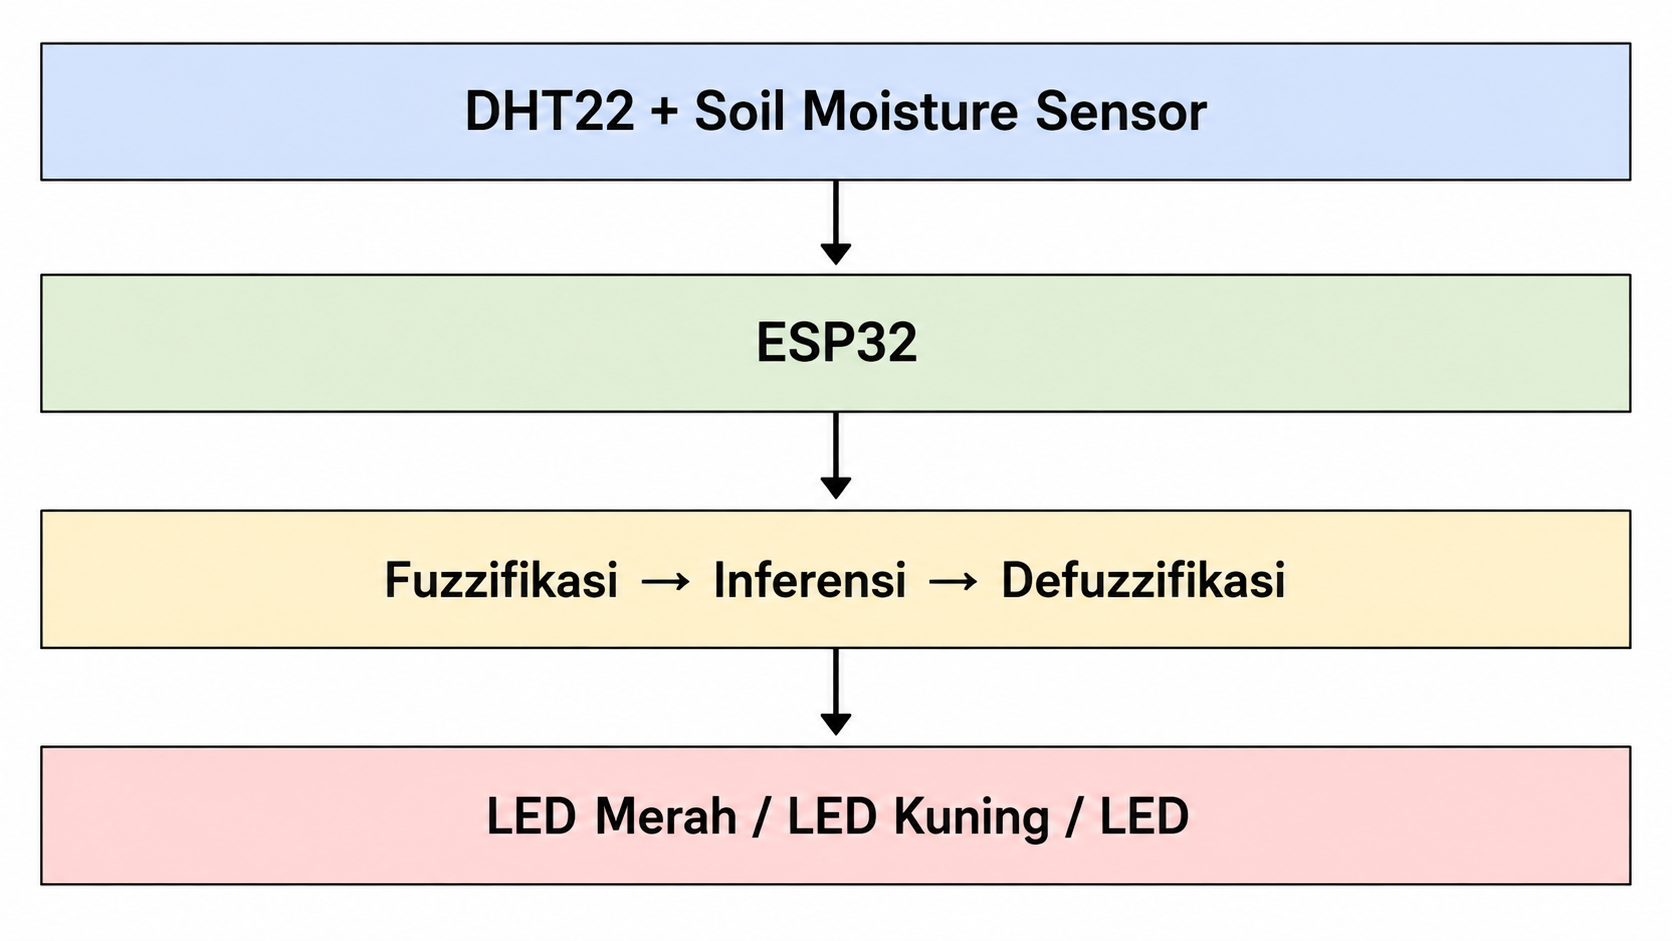
\includegraphics[width=0.6\textwidth]{images/diagram-blok-sistem.png}
    \caption{Diagram blok sistem percobaan}
    \label{fig:alur-fuzzy}
\end{figure}

Alur kerja sistem dimulai dari pembacaan data suhu dan kelembapan tanah oleh sensor. Data dari sensor kemudian diterima dan dibaca oleh ESP32, dengan nilai dari sensor analog dibaca menggunakan Analog to Digital Converter (ADC). Selanjutnya, data yang diperoleh diproses menggunakan logika fuzzy untuk menentukan kondisi sistem berdasarkan aturan yang telah dirancang. Hasil pengolahan tersebut kemudian digunakan untuk menentukan LED yang menyala sesuai dengan kondisi sistem.

\subsection{Perancangan Input dan Output}

Dua variabel digunakan sebagai masukan sistem, yaitu suhu dan kelembapan tanah. Masing-masing variabel dibagi menjadi tiga kategori untuk menyederhanakan proses pengambilan keputusan dan penyusunan rule. Setiap kategori memiliki batas nilai yang telah ditentukan sesuai dengan parameter yang digunakan pada sistem.

\begin{table}[H]
    \centering
    \caption{Kategori input sistem}
    \label{tab:kategoriinput}
    \begin{tabularx}{\textwidth}{p{0.25\textwidth} p{0.15\textwidth} X}
        \toprule
        \textbf{Variabel} & \textbf{Himpunan} & \textbf{Makna} \\
        \midrule
        Suhu & Rendah & Suhu relatif rendah untuk kondisi pengamatan \\
        Suhu & Sedang & Suhu relatif sesuai dengan kondisi pengamatan \\
        Suhu & Tinggi & Suhu relatif tinggi untuk kondisi pengamatan \\
        \midrule
        Kelembapan tanah & Kering & Media relatif kering \\
        Kelembapan tanah & Sedang & Media memiliki kelembapan menengah \\
        Kelembapan tanah & Lembap & Media relatif lembap \\
        \bottomrule
    \end{tabularx}
\end{table}

Output sistem terdiri dari tiga kategori yang digunakan untuk merepresentasikan hasil keputusan fuzzy. Nilai keluaran dari proses defuzzifikasi kemudian dipetakan ke kategori LED yang telah ditentukan, sehingga hasil keputusan dapat ditampilkan secara langsung.

\begin{table}[H]
    \centering
    \caption{Kategori output sistem}
    \label{tab:output}
    \begin{tabularx}{\textwidth}{c c c X}
        \toprule
        \textbf{Kategori} & \textbf{LED} & \textbf{Nilai Output} & \textbf{Makna} \\
        \midrule
        1 & Merah & 0 & Kondisi kurang sesuai \\
        2 & Kuning & 50 & Kondisi perlu diperhatikan \\
        3 & Hijau & 100 & Kondisi relatif baik \\
        \bottomrule
    \end{tabularx}
\end{table}

\subsection{Membership Function}

Membership function digunakan untuk mengubah nilai sensor menjadi derajat keanggotaan. Bentuk yang digunakan pada modul ini adalah fungsi keanggotaan segitiga karena dapat dihitung dengan langkah yang sederhana. Parameter pada tabel berikut adalah contoh rancangan awal dan bukan hasil kalibrasi aktual.

\begin{table}[H]
    \centering
    \caption{Contoh parameter membership function suhu}
    \label{tab:mfsuhu}
    \begin{tabularx}{\textwidth}{l c c c X}
        \toprule
        \textbf{Himpunan} & \textbf{a} & \textbf{b} & \textbf{c} & \textbf{Status} \\
        \midrule
        Rendah & 15 & 20 & 25 & \textbf{[CONTOH PARAMETER]} \\
        Sedang & 22 & 27 & 32 & \textbf{[CONTOH PARAMETER]} \\
        Tinggi & 29 & 34 & 39 & \textbf{[CONTOH PARAMETER]} \\
        \bottomrule
    \end{tabularx}
\end{table}

\begin{table}[H]
    \centering
    \caption{Contoh parameter membership function kelembapan tanah}
    \label{tab:mfsoil}
    \begin{tabularx}{\textwidth}{l c c c X}
        \toprule
        \textbf{Himpunan} & \textbf{a} & \textbf{b} & \textbf{c} & \textbf{Status} \\
        \midrule
        Kering & 0 & 20 & 40 & \textbf{[CONTOH PARAMETER]} \\
        Sedang & 30 & 50 & 70 & \textbf{[CONTOH PARAMETER]} \\
        Lembap & 60 & 80 & 100 & \textbf{[CONTOH PARAMETER]} \\
        \bottomrule
    \end{tabularx}
\end{table}



Penguji tidak perlu menghitung seluruh kombinasi membership function secara manual. Satu contoh perhitungan digunakan untuk memahami alur, sedangkan perhitungan pada program dapat dilakukan oleh ESP32.

\subsection{Fuzzy Rule}

Rule base dibuat dengan mempertimbangkan dua input utama. Pada kondisi suhu yang sesuai dan kelembapan tanah yang sesuai, keluaran diarahkan menuju kondisi relatif baik. Sebaliknya, kombinasi kondisi yang terlalu kering atau terlalu ekstrem diarahkan menuju indikator merah atau kuning.

\begin{table}[H]
    \centering
    \caption{Rule base}
    \label{tab:rulebase}
    \small
    \begin{tabularx}{\textwidth}{c L L L}
        \toprule
        \textbf{No.} & \textbf{Suhu} & \textbf{Kelembapan Tanah} & \textbf{Output} \\
        \midrule
        R1 & Rendah & Kering & Merah \\
        R2 & Rendah & Sedang & Kuning \\
        R3 & Rendah & Lembap & Kuning \\
        R4 & Sedang & Kering & Kuning \\
        R5 & Sedang & Sedang & Hijau \\
        R6 & Sedang & Lembap & Hijau \\
        R7 & Tinggi & Kering & Merah \\
        R8 & Tinggi & Sedang & Kuning \\
        R9 & Tinggi & Lembap & Kuning \\
        \bottomrule
    \end{tabularx}
\end{table}

Aturan R5 dapat dibaca sebagai: jika suhu berada pada kategori sedang dan kelembapan tanah berada pada kategori sedang, maka kondisi tanaman dinyatakan relatif baik. Aturan R7 menunjukkan bahwa kombinasi suhu tinggi dan media kering perlu diberi perhatian lebih besar sehingga indikator diarahkan ke merah. Aturan lain digunakan untuk menjaga agar kondisi antara tidak langsung dipetakan sebagai kondisi terbaik atau terburuk.
% =========================================================
% 6. PERCOBAAN 1
% =========================================================
\section{Percobaan 1: Pembacaan Kondisi Lingkungan}

Percobaan pertama dilakukan untuk memastikan bahwa sensor dapat digunakan sebagai sumber data sistem. Penguji mengamati nilai suhu dan kelembapan tanah sebelum proses pengambilan keputusan diaktifkan. Pada percobaan ini, perubahan kelembapan media dibuat menggunakan beberapa kondisi rockwool, sedangkan perubahan suhu diamati pada kondisi suhu ruangan dan saat media atau area sensor terkena udara panas dari hair dryer.

\subsection{Prosedur Percobaan}

\begin{enumerate}
    \item Siapkan ESP32, DHT22, capacitive soil moisture sensor, breadboard, kabel jumper, rockwool, dan hair dryer.
    \item Rangkai DHT22 dan soil moisture sensor sesuai konfigurasi yang digunakan.
    \item Hubungkan ESP32 ke laptop.
    \item Buka program pembacaan sensor.
    \item Sesuaikan nomor pin pada program dengan wiring aktual.
    \item Upload program ke ESP32.
    \item Buka Serial Monitor.
    \item Jalankan sistem pada kondisi suhu ruangan dan catat nilai suhu.
    \item Siapkan rockwool dalam kondisi kering tanpa tambahan air.
    \item Catat nilai pembacaan kelembapan tanah pada kondisi tersebut.
    \item Siapkan rockwool dalam kondisi normal dengan penambahan air sebanyak \textbf{[}\rule{1cm}{0.4pt}\textbf{ mL]}.
    \item Tunggu hingga air tersebar pada rockwool, kemudian catat nilai pembacaan kelembapan tanah.
    \item Siapkan rockwool dalam kondisi lembap dengan penambahan air sebanyak \textbf{[}\rule{1cm}{0.4pt}\textbf{ mL]}.
    \item Catat kembali nilai pembacaan kelembapan tanah.
    \item Uji kondisi suhu panas menggunakan hair dryer dengan jarak yang aman dari sensor dan komponen.
    \item Amati perubahan nilai suhu yang terbaca pada Serial Monitor.
    \item Catat seluruh hasil pengamatan.
\end{enumerate}

\begin{lstlisting}[language=C++, caption={Program pembacaan sensor untuk Percobaan 1}, label={lst:percobaan1}]
#include <Arduino.h>
#include <DHT.h>

#define DHT_PIN       4
#define DHT_TYPE      DHT22
#define SOIL_PIN      34

DHT dht(DHT_PIN, DHT_TYPE);

void setup()
{
    Serial.begin(115200);
    dht.begin();
}

void loop()
{
    float temperature = dht.readTemperature();
    int soilRaw = analogRead(SOIL_PIN);

    if (isnan(temperature)) {
        Serial.println("Pembacaan DHT22 gagal.");
        delay(1000);
        return;
    }

    Serial.print("Suhu: ");
    Serial.print(temperature);
    Serial.print(" C | Soil Raw: ");
    Serial.println(soilRaw);

    delay(1000);
}
\end{lstlisting}

\placeholderfigure{5cm}{[GAMBAR: Wiring sensor DHT22 dan Capacitive Soil Moisture Sensor]}

\placeholderfigure{4cm}{[GAMBAR: Tampilan pembacaan sensor pada Serial Monitor]}

\subsection{Analisis Percobaan}

Analisis dilakukan dengan membandingkan pembacaan sensor pada kondisi rockwool yang berbeda dan pada kondisi suhu yang berbeda. Perhatikan perubahan nilai kelembapan tanah ketika rockwool berada pada kondisi kering, normal, dan lembap. Selain itu, amati perubahan suhu yang terbaca ketika sistem berada pada suhu ruangan dan ketika terkena udara panas dari hair dryer.

\subsubsection*{Target Pengamatan}

\begin{itemize}
    \item [ ] Data suhu dapat terbaca pada Serial Monitor.
    \item [ ] Data kelembapan tanah dapat terbaca.
    \item [ ] Nilai sensor kelembapan berubah pada setiap kondisi rockwool.
    \item [ ] Nilai suhu berubah ketika sensor terkena udara panas dari hair dryer.
    \item [ ] Pembacaan sensor dapat digunakan sebagai input sistem.
    \item [ ] Tidak terdapat pembacaan sensor yang tidak wajar selama pengamatan.
\end{itemize}

\subsubsection*{Catatan}

\noindent
\makebox[\textwidth]{\hrulefill}

\vspace{0.4cm}
\makebox[\textwidth]{\hrulefill}

\vspace{0.4cm}
\makebox[\textwidth]{\hrulefill}

% =========================================================
% 7. PERCOBAAN 2
% =========================================================
\section{Percobaan 2: Implementasi Metode Pengambilan Keputusan}

Percobaan kedua menggabungkan pembacaan sensor dengan proses pengambilan keputusan. Nilai sensor digunakan sebagai input untuk membership function dan rule yang telah dirancang. Hasil pengolahan ditampilkan melalui LED agar perubahan keputusan dapat diamati secara langsung.

\subsection{Prosedur Percobaan}

\begin{enumerate}
    \item Lanjutkan dari rangkaian Percobaan 1.
    \item Pastikan seluruh koneksi sensor masih terpasang dengan benar.
    \item Tambahkan tiga LED sebagai indikator keluaran.
    \item Pasang resistor LED sesuai kebutuhan rangkaian.
    \item Masukkan parameter membership function ke dalam program.
    \item Masukkan rule base ke dalam program.
    \item Upload program ke ESP32.
    \item Jalankan sistem pada kondisi suhu ruangan.
    \item Uji kondisi rockwool kering tanpa tambahan air.
    \item Amati nilai sensor dan LED yang aktif.
    \item Uji kondisi rockwool normal dengan penambahan air sebanyak \textbf{[}\underline{\phantom{mL}}\textbf{mL]}.
    \item Amati perubahan nilai sensor dan LED.
    \item Uji kondisi rockwool lembap dengan penambahan air sebanyak \textbf{[}\underline{\phantom{mL}}\textbf{mL]}.
    \item Amati kembali perubahan nilai sensor dan LED.
    \item Uji kondisi suhu panas menggunakan hair dryer dengan jarak yang aman.
    \item Amati perubahan suhu, nilai keluaran, dan LED yang aktif.
\end{enumerate}

\begin{lstlisting}[language=C++, caption={Program implementasi fuzzy logic untuk Percobaan 2}, label={lst:percobaan2}]
#include <Arduino.h>
#include <DHT.h>

#define DHT_PIN       4
#define DHT_TYPE      DHT22
#define SOIL_PIN      34

#define LED_RED       25
#define LED_YELLOW    26
#define LED_GREEN     27

DHT dht(DHT_PIN, DHT_TYPE);

float trimf(float x, float a, float b, float c)
{
    if (x <= a || x >= c) {
        return 0.0;
    }

    if (x == b) {
        return 1.0;
    }

    if (x < b) {
        return (x - a) / (b - a);
    }

    return (c - x) / (c - b);
}

void setLED(int outputClass)
{
    digitalWrite(LED_RED, LOW);
    digitalWrite(LED_YELLOW, LOW);
    digitalWrite(LED_GREEN, LOW);

    if (outputClass == 0) {
        digitalWrite(LED_RED, HIGH);
    }
    else if (outputClass == 50) {
        digitalWrite(LED_YELLOW, HIGH);
    }
    else if (outputClass == 100) {
        digitalWrite(LED_GREEN, HIGH);
    }
}

void setup()
{
    Serial.begin(115200);
    dht.begin();

    pinMode(LED_RED, OUTPUT);
    pinMode(LED_YELLOW, OUTPUT);
    pinMode(LED_GREEN, OUTPUT);

    setLED(50);
}

void loop()
{
    float temperature = dht.readTemperature();
    int soilRaw = analogRead(SOIL_PIN);

    if (isnan(temperature)) {
        Serial.println("Pembacaan DHT22 gagal.");
        delay(1000);
        return;
    }

    /*
     * Skala soilRaw perlu disesuaikan berdasarkan
     * hasil pengukuran sensor aktual.
     */
    float soilValue = map(soilRaw, 4095, 0, 0, 100);

    // Membership suhu.
    float tempLow  = trimf(temperature, 15, 20, 25);
    float tempMed  = trimf(temperature, 20, 25, 30);
    float tempHigh = trimf(temperature, 25, 30, 35);

    // Membership kelembapan tanah.
    float soilDry  = trimf(soilValue, 0, 20, 40);
    float soilMed  = trimf(soilValue, 30, 50, 70);
    float soilWet  = trimf(soilValue, 60, 80, 100);

    // Kekuatan rule.
    float r1 = min(tempLow,  soilDry);
    float r2 = min(tempLow,  soilMed);
    float r3 = min(tempLow,  soilWet);

    float r4 = min(tempMed,  soilDry);
    float r5 = min(tempMed,  soilMed);
    float r6 = min(tempMed,  soilWet);

    float r7 = min(tempHigh, soilDry);
    float r8 = min(tempHigh, soilMed);
    float r9 = min(tempHigh, soilWet);

    /*
     * Output singleton:
     * Merah  = 0
     * Kuning = 50
     * Hijau  = 100
     */
    float weightedOutput =
        (r1 * 0)  +
        (r2 * 50) +
        (r3 * 50) +
        (r4 * 50) +
        (r5 * 100) +
        (r6 * 100) +
        (r7 * 0) +
        (r8 * 50) +
        (r9 * 50);

    float totalRule =
        r1 + r2 + r3 +
        r4 + r5 + r6 +
        r7 + r8 + r9;

    if (totalRule <= 0.0) {
        Serial.println("Tidak ada rule aktif.");
        setLED(50);
    }
    else {
        float output = weightedOutput / totalRule;

        if (output < 25) {
            setLED(0);
        }
        else if (output < 75) {
            setLED(50);
        }
        else {
            setLED(100);
        }

        Serial.print("Suhu: ");
        Serial.print(temperature);
        Serial.print(" C | Soil: ");
        Serial.print(soilValue);
        Serial.print(" | Output: ");
        Serial.println(output);
    }

    delay(1000);
}
\end{lstlisting}

\placeholderfigure{5cm}{[GAMBAR: Wiring lengkap ESP32, DHT22, Soil Moisture Sensor, dan LED]}

\subsection{Analisis Percobaan}

Analisis pada percobaan kedua berfokus pada hubungan antara perubahan input dan keluaran sistem. Perhatikan perubahan LED pada kondisi rockwool yang berbeda serta perubahan keluaran ketika suhu meningkat akibat penggunaan hair dryer. Hasil pengamatan dibandingkan dengan kecenderungan yang dihasilkan oleh rule yang telah dibuat.

\subsubsection*{Target Pengamatan}

\begin{itemize}
    \item [ ] Nilai sensor dapat diproses menggunakan membership function.
    \item [ ] Rule dapat digunakan untuk menghasilkan keluaran.
    \item [ ] Output berubah ketika kondisi rockwool berubah.
    \item [ ] Output berubah ketika suhu meningkat.
    \item [ ] LED menyala sesuai dengan hasil pengolahan.
    \item [ ] Hasil aktual mengikuti kecenderungan yang diprediksi.
    \item [ ] Sistem tidak menghasilkan kondisi output yang tidak didefinisikan.
\end{itemize}

\subsubsection*{Catatan}

\noindent
\makebox[\textwidth]{\hrulefill}

\vspace{0.4cm}
\makebox[\textwidth]{\hrulefill}

\vspace{0.4cm}
\makebox[\textwidth]{\hrulefill}

% =========================================================
% 8. PERCOBAAN 3
% =========================================================
\section{Percobaan 3: Pengujian Kondisi Lingkungan}

Percobaan ketiga digunakan untuk menguji respons akhir sistem terhadap beberapa kombinasi kondisi lingkungan. Program yang digunakan sama dengan program pada Percobaan 2 sehingga pengujian difokuskan pada pengamatan hubungan antara kondisi rockwool, suhu, dan keluaran LED.

\subsection{Prosedur Percobaan}

\begin{enumerate}
    \item Pastikan sistem pada Percobaan 2 telah berjalan.
    \item Gunakan program yang sama dengan Percobaan 2.
    \item Siapkan rockwool dalam kondisi kering tanpa tambahan air.
    \item Amati suhu ruangan, nilai kelembapan tanah, dan LED yang aktif.
    \item Catat hasil pada Tabel~\ref{tab:pengamatan}.
    \item Siapkan rockwool dalam kondisi normal dengan penambahan air sebanyak \textbf{[\underline{\phantom{0000}} mL]}.
    \item Amati kembali nilai sensor dan LED.
    \item Siapkan rockwool dalam kondisi lembap dengan penambahan air sebanyak \textbf{[\underline{\phantom{0000}} mL]}.
    \item Amati kembali nilai sensor dan LED.
    \item Gunakan hair dryer untuk menghasilkan kondisi suhu yang lebih tinggi dengan jarak yang aman.
    \item Amati perubahan suhu dan LED pada kondisi rockwool yang sama.
    \item Bandingkan hasil setiap kondisi dengan kecenderungan rule.
\end{enumerate}

\subsubsection*{Kondisi A: Suhu Ruangan dan Rockwool Kering}

Kondisi pertama digunakan untuk melihat respons sistem pada suhu ruangan dengan media yang tidak diberi tambahan air. Hasil pembacaan sensor dan LED digunakan sebagai kondisi awal pembanding.

\subsubsection*{Kondisi B: Suhu Ruangan dan Rockwool Normal}

Kondisi kedua digunakan untuk melihat perubahan sistem setelah rockwool diberi air sebanyak \textbf{[\underline{\phantom{0000}} mL]}. Hasil pengamatan dibandingkan dengan kondisi rockwool kering.

\subsubsection*{Kondisi C: Suhu Ruangan dan Rockwool Lembap}

Kondisi ketiga digunakan untuk melihat respons sistem pada rockwool dengan kandungan air yang lebih tinggi, yaitu setelah diberi air sebanyak \textbf{[\underline{\phantom{0000}} mL]}. Hasil keluaran dibandingkan dengan kondisi sebelumnya.

\subsubsection*{Kondisi D: Suhu Panas dan Rockwool Tetap}

Kondisi keempat digunakan untuk melihat pengaruh kenaikan suhu terhadap hasil pengambilan keputusan. Suhu dinaikkan menggunakan hair dryer dengan jarak yang aman dan rockwool dipertahankan pada kondisi yang sama selama pengamatan.

\subsection{Tabel Pengamatan}

\begin{table}[H]
    \centering
    \caption{Tabel pengamatan kondisi lingkungan}
    \label{tab:pengamatan}
    \small
    \begin{tabularx}{\textwidth}{c L c c c c L}
        \toprule
        \textbf{No.} &
        \textbf{Kondisi} &
        \textbf{Suhu} &
        \textbf{Kelembapan Tanah} &
        \textbf{Prediksi} &
        \textbf{LED Aktual} &
        \textbf{Catatan} \\
        \midrule
        1 & Suhu ruangan + rockwool kering & & & & & \\
        2 & Suhu ruangan + rockwool normal & & & & & \\
        3 & Suhu ruangan + rockwool lembap & & & & & \\
        4 & Suhu panas + rockwool tetap & & & & & \\
        \bottomrule
    \end{tabularx}
\end{table}

\textbf{[DATA AKTUAL DIPERLUKAN]}

Nilai pada tabel harus diisi berdasarkan hasil pengukuran langsung selama percobaan. Jangan menggunakan nilai pada contoh perhitungan sebagai data pengamatan. Catatan harus menunjukkan kondisi yang benar-benar terlihat pada saat sistem dijalankan.

\subsection{Analisis Percobaan}

Analisis dilakukan dengan membandingkan perubahan input terhadap perubahan output sistem. Perhatikan pengaruh kondisi rockwool terhadap nilai kelembapan tanah serta pengaruh peningkatan suhu terhadap hasil pengambilan keputusan. Hasil pengamatan kemudian dibandingkan dengan kecenderungan yang diharapkan berdasarkan membership function dan rule yang telah dirancang.

\subsubsection*{Target Pengamatan}

\begin{itemize}
    \item [ ] Sistem dapat membaca kondisi rockwool yang berbeda.
    \item [ ] Perubahan kelembapan rockwool memengaruhi hasil pengolahan.
    \item [ ] Peningkatan suhu memengaruhi hasil pengolahan.
    \item [ ] Output berubah mengikuti perubahan kondisi input.
    \item [ ] LED menunjukkan kondisi sesuai rancangan.
    \item [ ] Hasil pengamatan secara umum sesuai dengan prediksi.
    \item [ ] Tidak terdapat keluaran yang bertentangan dengan rule.
\end{itemize}

\subsubsection*{Catatan}

\noindent
\makebox[\textwidth]{\hrulefill}

\vspace{0.4cm}
\makebox[\textwidth]{\hrulefill}

\vspace{0.4cm}
\makebox[\textwidth]{\hrulefill}

% =========================================================
% 9. MINI CHALLENGE
% =========================================================
\section{Mini Challenge}

\textbf{Kasus: ``LED kuning terlalu sering menyala.''}

Sistem telah bekerja, tetapi LED kuning muncul lebih sering daripada yang diperkirakan. Kondisi tersebut dapat terjadi karena batas kategori input terlalu lebar, rule terlalu konservatif, atau perubahan pembacaan sensor membuat sistem sering berada pada kondisi antara. Penguji diminta mencari satu bagian rancangan yang paling mungkin menyebabkan kondisi tersebut dan mencoba melakukan penyesuaian.

\subsection*{Tugas}

Lakukan satu perubahan pada salah satu bagian berikut:
\begin{itemize}
    \item parameter membership function;
    \item rule base;
    \item batas pemetaan output LED.
\end{itemize}

Setelah perubahan dilakukan, jalankan sistem kembali dan bandingkan hasil sebelum dan sesudah perubahan. Perubahan harus dicatat agar penguji dapat melihat bahwa rancangan pengambilan keputusan memengaruhi perilaku keluaran.

\subsection*{Target Challenge}

\begin{itemize}
    \item [ ] Penyebab kemungkinan LED kuning terlalu sering menyala dapat diidentifikasi.
    \item [ ] Minimal satu parameter atau rule diubah.
    \item [ ] Program berhasil diunggah kembali.
    \item [ ] Perilaku LED berubah setelah modifikasi.
    \item [ ] Perubahan hasil dapat dijelaskan berdasarkan bagian sistem yang diubah.
\end{itemize}

\subsubsection*{Perubahan yang Dilakukan}

\noindent
\makebox[\textwidth]{\hrulefill}

\vspace{0.4cm}
\makebox[\textwidth]{\hrulefill}

\subsubsection*{Hasil Setelah Perubahan}

\noindent
\makebox[\textwidth]{\hrulefill}

\vspace{0.4cm}
\makebox[\textwidth]{\hrulefill}

% =========================================================
% 10. PENUTUP
% =========================================================
\section{Penutup}

Pada percobaan ini, penguji telah menggunakan data suhu dan kelembapan tanah sebagai input sistem monitoring kondisi tanaman. Data sensor diproses menggunakan membership function dan rule sederhana untuk menghasilkan keputusan yang kemudian ditampilkan melalui LED. Rangkaian tersebut menunjukkan bagaimana metode pengambilan keputusan dapat diimplementasikan secara langsung pada ESP32 sebagai platform embedded system.

Melalui tiga percobaan, penguji mengamati pembacaan sensor, implementasi pengolahan, dan respons sistem terhadap beberapa kondisi lingkungan. Hasil pengamatan dapat digunakan untuk menilai apakah parameter dan rule yang dirancang telah memberikan keluaran sesuai dengan tujuan awal. Mini challenge kemudian menunjukkan bahwa perubahan rancangan dapat memengaruhi perilaku sistem sehingga parameter perlu diuji dan disesuaikan berdasarkan hasil pengamatan.

\end{document}